\chapter{Forsøg 1} \label{bilag:forsg1}

\begin{figure}[H]
\centering
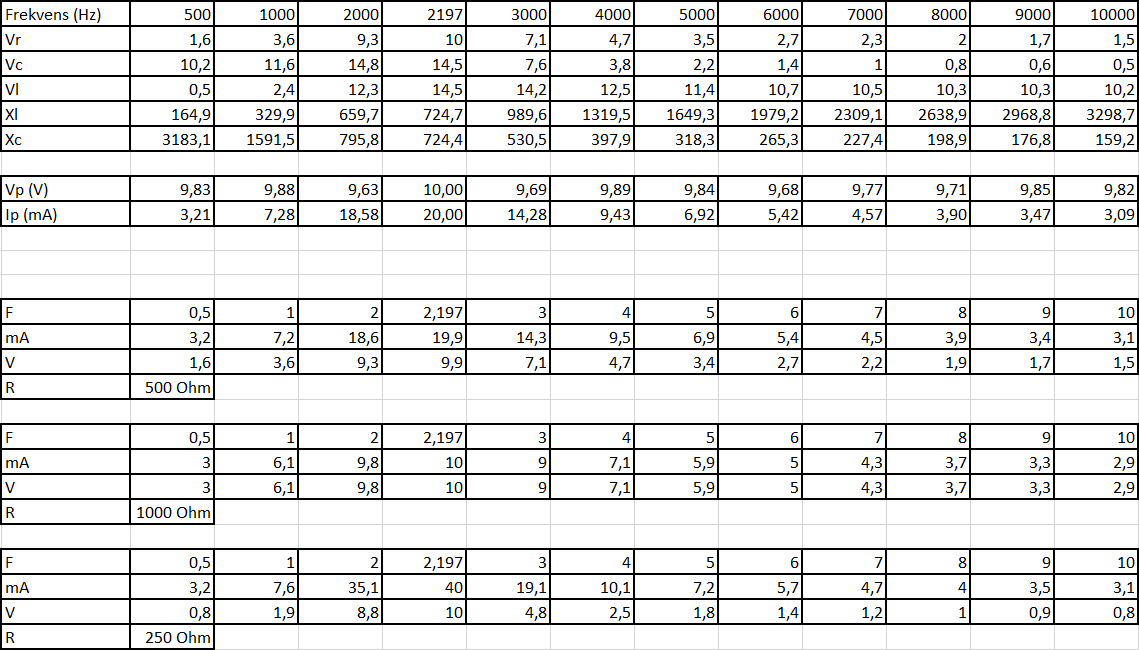
\includegraphics[width=1\textwidth]{Setup/Bilag_forsg1}
\caption{Rå data for forsøg 1}
\label{tabular:forsg1}
\end{figure}

\textbf{RC - kredsløb}

\begin{figure}[H]
	\centering
	\begin{minipage}[b]{0.48\textwidth}
	\centering
	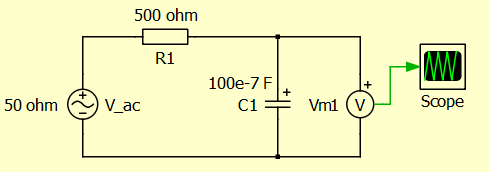
\includegraphics[width=1\textwidth]{Vildledning/Schematics/kredslb/RC} % Venstre billede
	\end{minipage}
	\hfill
	\begin{minipage}[b]{0.48\textwidth}
	\centering
	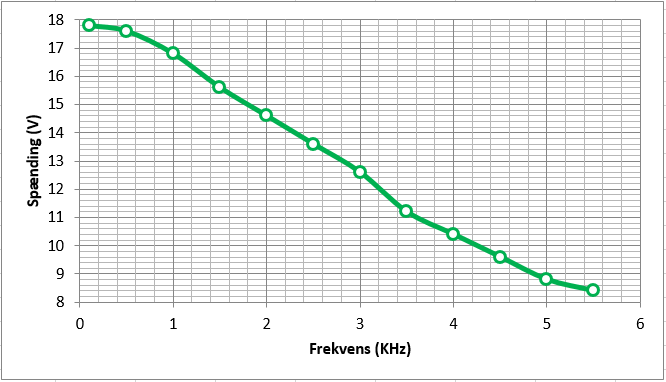
\includegraphics[width=1\textwidth]{Setup/Graf1} % Højre billede
	\end{minipage}
	\\ % Figurtekster og labels
	\begin{minipage}[t]{0.48\textwidth}
	\caption{Opstilling af RC-kredsløb} % Venstre figurtekst og label
	\end{minipage}
	\hfill
	\begin{minipage}[t]{0.48\textwidth}
	\caption{Graf for RC-kredsløb} % Højre figurtekst og label
	\end{minipage}
\end{figure}
\newpage

\textbf{RL - Kredsløb}

\begin{figure}[H]
	\centering
	\begin{minipage}[b]{0.48\textwidth}
	\centering
	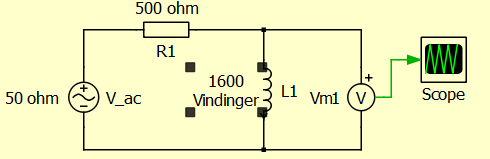
\includegraphics[width=1\textwidth]{Vildledning/Schematics/kredslb/RL} % Venstre billede
	\end{minipage}
	\hfill
	\begin{minipage}[b]{0.48\textwidth}
	\centering
	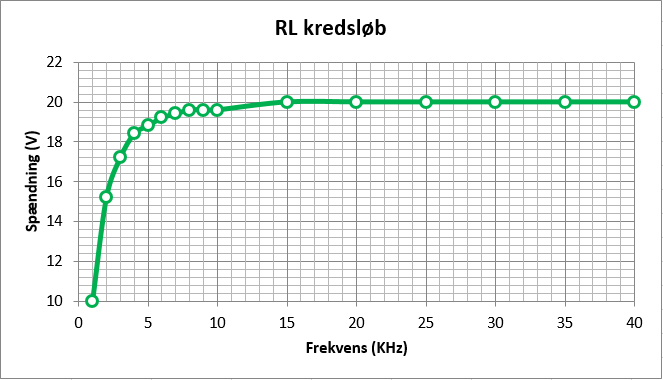
\includegraphics[width=1\textwidth]{Setup/Graf2} % Højre billede
	\end{minipage}
	\\ % Figurtekster og labels
	\begin{minipage}[t]{0.48\textwidth}
	\caption{Opstilling af RL-kredsløb} % Venstre figurtekst og label
	\end{minipage}
	\hfill
	\begin{minipage}[t]{0.48\textwidth}
	\caption{Graf for RL-kredsløb} % Højre figurtekst og label
	\end{minipage}
\end{figure}

\textbf{CL - Kredsløb Serie}

\begin{figure}[H]
	\centering
	\begin{minipage}[b]{0.48\textwidth}
	\centering
	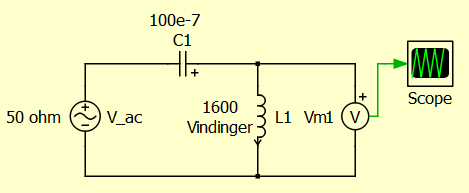
\includegraphics[width=1\textwidth]{Vildledning/Schematics/kredslb/CL_serie} % Venstre billede
	\end{minipage}
	\hfill
	\begin{minipage}[b]{0.48\textwidth}
	\centering
	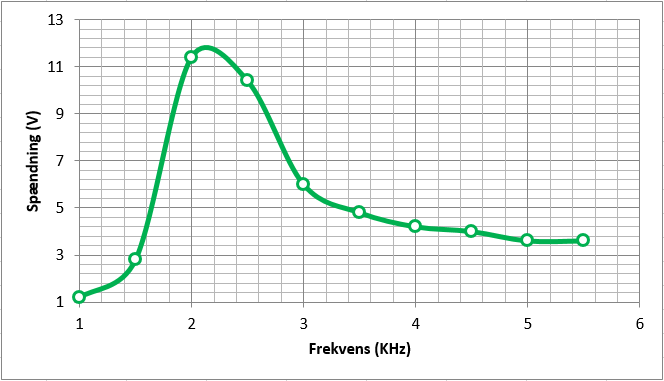
\includegraphics[width=1\textwidth]{Setup/Graf4} % Højre billede
	\end{minipage}
	\\ % Figurtekster og labels
	\begin{minipage}[t]{0.48\textwidth}
	\caption{Opstilling af CL-kredsløb} % Venstre figurtekst og label
	\end{minipage}
	\hfill
	\begin{minipage}[t]{0.48\textwidth}
	\caption{Graf for CL-kredsløb} % Højre figurtekst og label
	\end{minipage}
\end{figure}

\textbf{LC - Kredsløb Parallel}

\begin{figure}[H]
	\centering
	\begin{minipage}[b]{0.48\textwidth}
	\centering
	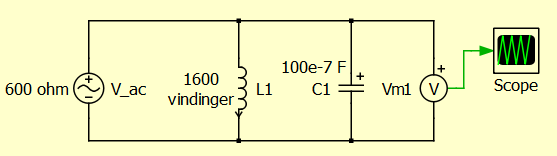
\includegraphics[width=1\textwidth]{Vildledning/Schematics/kredslb/LC_Parallel} % Venstre billede
	\end{minipage}
	\hfill
	\begin{minipage}[b]{0.48\textwidth}
	\centering
	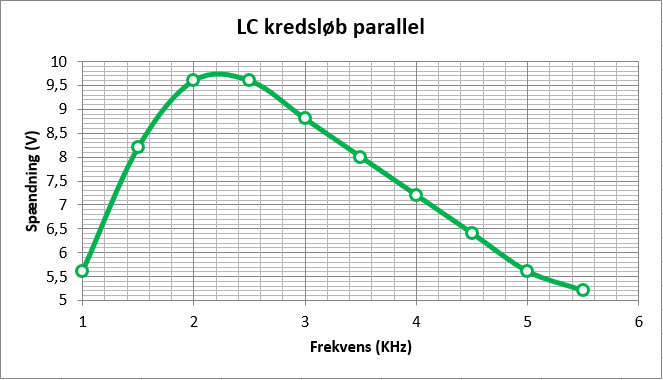
\includegraphics[width=1\textwidth]{Setup/Graf5} % Højre billede
	\end{minipage}
	\\ % Figurtekster og labels
	\begin{minipage}[t]{0.48\textwidth}
	\caption{Opstilling af LC-kredsløb parallel} % Venstre figurtekst og label
	\end{minipage}
	\hfill
	\begin{minipage}[t]{0.48\textwidth}
	\caption{Graf for LC-kredsløb parallel} % Højre figurtekst og label
	\end{minipage}
\end{figure}